\documentclass{article}

\usepackage{defines}

\usepackage{tikz, caption}

\begin{document}

\tickettitle{3}{Геометрический смысл линейной зависимости и независимости векторов. Теоремы о необходимых и достаточных условиях линейной зависимости векторов в $V^{2}$ и $V^{3}$. Следствия.}

\theorem
\begin{align*}
	\{\vec{a},\vec{b}\}\text{ --- лз}\Lrarr \vec{a}\parallel\vec{b}
\end{align*}

\onlyif
\begin{align*}
	 & \lambda_1\vec{a}+\lambda_2\vec{b}=\vec{0} &  & \exists i:\lambda_{i}\neq 0
\end{align*}

Без ограничения общности пусть $\lambda_{1}\neq 0$, тогда:
\begin{align*}
	\lambda_1\vec{a}+\lambda_2\vec{b}=\vec{0}\Rarr\vec{a}+\frac{\lambda_2}{\lambda_1}\vec{b}=\vec{0}\Rarr\vec{a}=-\frac{\lambda_2}{\lambda_1}\vec{b}\Rarr\vec{a}\parallel\vec{b}\qed
\end{align*}

\enough
\begin{align*}
	 & \vec{a}\parallel\vec{b}\Rarr\exists\lambda\in\R:\vec{a}=\lambda\vec{b}                   \\
	 & \vec{a}=\lambda\vec{b}\Rarr(-1)\vec{a}+\lambda\vec{b}=0,\;(-1)^{2}+\lambda^{2}\neq 0\qed
\end{align*}

\result[1]

Обратив утверждение получаем:
\begin{align*}
	\{\vec{a},\vec{b}\}\text{ --- лнз}\Lrarr \vec{a}\nparallel\vec{b}
\end{align*}

\theorem
\begin{align*}
	\{\vec{a},\vec{b},\vec{c}\}\text{ --- лз}\Lrarr \{\vec{a},\vec{b},\vec{c}\}\text{ --- компланарны}
\end{align*}

\onlyif
\begin{align*}
	\alpha\vec{a}+\beta\vec{b}+\gamma\vec{c}=\vec{0}
\end{align*}

Без ограничения общности пусть $\gamma\neq 0$, тогда:
\begin{align*}
	\alpha\vec{a}+\beta\vec{b}+\gamma\vec{c}=\vec{0}\Rarr
	\frac{\alpha}{\gamma}\vec{a}+\frac{\beta}{\gamma}\vec{b}+\vec{c}=\vec{0}\Rarr
	\vec{c}=\left(-\frac{\alpha}{\gamma}\right)\vec{a}+\left(-\frac{\beta}{\gamma}\right)\vec{b}
\end{align*}

$\vec{c}$ --- линейная комбинация $\vec{a}$ и $\vec{b}$ $\Rarr$ $\{\vec{a},\vec{b},\vec{c}\}$ --- компланарны$\qed$

\pagebreak

\enough
\begin{minipage}{0.6\linewidth}
	\begin{enumerate}
		\item{}Приведём $\vec{a}$, $\vec{b}$, $\vec{c}$ к общему началу $O$.
		\item{}$C:\lvec{OC}=\vec{c}$
		\item{}$A=O\vec{a}\cap C\vec{b}$
		\item{}$B=O\vec{b}\cap C\vec{a}$
		\item{}$\lvec{OA}\parallel\vec{a}\Rarr\exists\alpha\in\R:\lvec{OA}=\alpha\vec{a}$
		\item{}$\lvec{OB}\parallel\vec{b}\Rarr\exists\beta\in\R:\lvec{OB}=\beta\vec{b}$
		\item{}$\lvec{BC}=\lvec{OA}$ (по свойству параллелограмма)
		\item{}$\vec{c}=\lvec{OC}=\lvec{OB}+\lvec{BC}=\lvec{OB}+\lvec{OA}=\alpha\vec{a}+\beta\vec{b}$
	\end{enumerate}
\end{minipage}%
\begin{minipage}{0.4\linewidth}
	\centering
	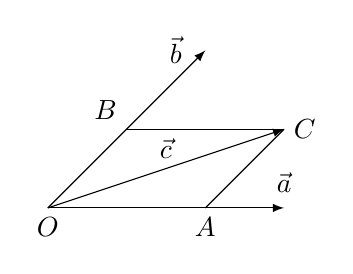
\begin{tikzpicture}
		\filldraw (0,0) node[anchor=north] {$O$};
		\filldraw (2,0) node[anchor=north] {$A$};
		\filldraw (1,1) node[anchor=south east] {$B$};
		\filldraw (3,1) node[anchor=west] {$C$};
		\draw [-latex] (0,0)--(3,0) node[above=0.2em] {$\vec{a}$};
		\draw [-latex] (0,0)--(2,2) node[left=0.5em] {$\vec{b}$};
		\draw [-latex] (0,0)--(3,1) node[midway, above] {$\vec{c}$};
		\draw (3,1)--(2,0);
		\draw (3,1)--(1,1);
	\end{tikzpicture}
	\captionof{figure}{Выражение $\vec{c}$ через $\vec{a}$ и $\vec{b}$}
\end{minipage}
\begin{align}
	 & \vec{c}=\alpha\vec{a}+\beta\vec{b}\Rarr(-1)\vec{c}+\alpha\vec{a}+\beta\vec{b}=\vec{0}\label{3:lcomb_1} \\
	 & (-1)^{2}+\alpha^{2}+\beta^{2}\neq 0\label{3:lcomb_2}
\end{align}
\begin{align*}
	\eqref{3:lcomb_1}\land\eqref{3:lcomb_2}\Rarr\{\vec{a},\vec{b},\vec{c}\}\text{ --- лз}\qed
\end{align*}

\result[1]

Обратив утверждение получаем:
\begin{align*}
	\{\vec{a},\vec{b},\vec{c}\}\text{ --- лнз}\Lrarr \{\vec{a},\vec{b},\vec{c}\}\text{ --- не компланарны}
\end{align*}

\result[2]

Среди трёх некомпланарных векторов не может быть $\vec{0}$ и коллинеарных пар.

\result[3]
\begin{align*}
	\vec{a}\nparallel\vec{b} \Rarr (\forall \vec{c}:\{\vec{a},\vec{b},\vec{c}\}\text {--- компланарны})\;\exists\alpha,\beta\in\R:\vec{c}=\alpha\vec{a}+\beta\vec{b}
\end{align*}

\pagebreak

\theorem

Любая система из четырёх векторов лз в $V^{3}$.

\proof
\begin{minipage}{0.6\linewidth}
	\begin{enumerate}
		\item{}Приведём $\vec{a}$, $\vec{b}$, $\vec{c}$, $\vec{d}$ к общему началу $O$.
		\item{}$D:\lvec{OD}=\vec{d}$
		\item{}$D'=O\vec{a}\vec{b}\cap D\vec{c}$
		\item{}$\vec{d}'=\lvec{OD'}$
		\item{}$\vec{d}',\vec{a},\vec{b}\text{ --- компланарны}\Rarr \exists\alpha,\beta\in\R:\vec{d}'=\alpha\vec{a}+\beta\vec{b}$
		\item{}$\lvec{D'D}\parallel\vec{c}\Rarr\exists\gamma\in\R:\lvec{D'D}=\gamma\vec{c}$
		\item{}$\vec{d}=\lvec{OD}=\lvec{OD'}+\lvec{D'D}=\vec{d}'+\gamma\vec{c}=\alpha\vec{a}+\beta\vec{b}+\gamma\vec{c}$
	\end{enumerate}
\end{minipage}%
\begin{minipage}{0.4\linewidth}
	\centering
	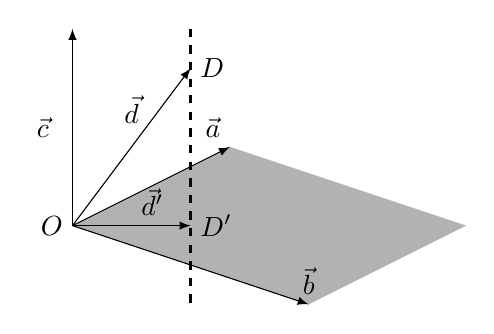
\begin{tikzpicture}
		\filldraw (0,0) node[anchor=east] {$O$};
		\filldraw (1.5,2) node[anchor=west] {$D$};
		\filldraw (1.5,0) node[anchor=west] {$D'$};
		\draw [-latex] (0,0)--(2,1) node[above left] {$\vec{a}$};
		\draw [-latex] (0,0)--(3,-1) node[above] {$\vec{b}$};
		\draw [-latex] (0,0)--(0,2.5) node[midway, left=0.5em] {$\vec{c}$};
		\draw [-latex] (0,0)--(1.5,2) node[midway, above=0.5em] {$\vec{d}$};
		\draw [-latex] (0,0)--(1.5,0) node[midway, above right] {$\vec{d}'$};
		\draw [dashed, thick] (1.5,2.5)--(1.5,-1);
		\fill [opacity=0.3] (0,0)--(2,1)--(5,0)--(3,-1)--cycle;
	\end{tikzpicture}
	\captionof{figure}{Выражение $\vec{d}$ через $\vec{a}$, $\vec{b}$ и $\vec{c}$}
\end{minipage}
\begin{align}
	 & \vec{d}=\alpha\vec{a}+\beta\vec{b}+\gamma\vec{c}\Rarr(-1)\vec{d}+\alpha\vec{a}+\beta\vec{b}+\gamma\vec{c}=\vec{0}\label{3:lcomb_3} \\
	 & (-1)^{2}+\alpha^{2}+\beta^{2}+\gamma^{2}\neq 0\label{3:lcomb_4}
\end{align}
\begin{align*}
	\eqref{3:lcomb_3}\land\eqref{3:lcomb_4}\Rarr\{\vec{a},\vec{b},\vec{c},\vec{d}\}\text{ --- лз}\qed
\end{align*}

\result[1]

Имея 3 некомпланарных вектора можно выразить четвёртый (в $V^{3}$).

\sectitle{Выводы}

\begin{enumerate}
	\item{}2 вектора в $V^{1}$ лз
	\item{}3 вектора в $V^{2}$ лз
	\item{}4 вектора в $V^{3}$ лз
	\item{}$\{\vec{a}\}$ --- лнз, если $\vec{a}\neq \vec{0}$
	\item{}$\vec{a}\nparallel\vec{b}\land\{\vec{a},\vec{b},\vec{c}\}\text{ --- компланарны}\Rarr\exists\alpha,\beta\in\R:\vec{c}=\alpha\vec{a}+\beta\vec{b}$
	\item{}$\{\vec{a},\vec{b},\vec{c}\}\text{ --- некомпланарны}\land\vec{a},\vec{b},\vec{c},\vec{d}\in V^{3}\Rarr\exists\alpha,\beta,\gamma\in\R:\vec{d}=\alpha\vec{a}+\beta\vec{b}+\gamma\vec{c}$
\end{enumerate}

\end{document}
